\appendix

\section{Description of datasets}

Most of the VQA datasets have strong biases. This allow models to learn strategies without reasoning about the visual input~\cite{Santoro2017ASN}.
The CLEVR dataset~\cite{johnson2017clevr} was developed to address those issues and come back to the core challenge of visual QA which is reasoning.
CLEVR contains images of 3D-rendered objects; each image comes with a number of highly compositional questions that fall into different categories.
Those categories fall into 5 classes of tasks: Exist, Count, Compare Integer, Query Attribute and Compare Attribute. 
The CLEVR dataset consists of:
\begin{itemize}
\item 	A training set of 70k images and 700k questions,
\item	A validation set of 15k images and 150k questions,
\item	A test  set of 15k images and 150k questions about objects,
\item	Answers, scene graphs and functional programs for all train and val images and questions.
\end{itemize}
Each object present in the scene, aside of position, is characterized by a set of four attributes:
\begin{itemize}
\item 2 sizes: large, small,
\item 3 shapes: square, cylinder, sphere,
\item 2 material types: rubber, metal,
\item 8 color types: gray, blue, brown, yellow, red, green, purple, cyan,
\end{itemize}
resulting in 96 unique combinations.

Along with CLEVR, the authors~\cite{johnson2017clevr} introduced  CLEVR-CoGenT (Compositional Generalization Test, CoGenT in short), with a goal of testing how well the models can learn and generalize compositional concepts.
This dataset is synthesized in the same way as CLEVR, but contains two conditions.
As shown in \tableref{tab:cogent_conditions}, in Condition A all cubes are gray, blue, brown, or yellow, whereas all cylinders are red, green, purple, or cyan; in Condition B cubes and cylinders swap color palettes.
Both conditions contain spheres of all colors.
CoGenT thus indicates how a model answers CLEVR questions: by memorizing combinations of traits or by learning disentangled or general representations.
The CoGenT dataset contains:
\begin{itemize}
\item	A training set of 70,000 images and 699,960 questions in Condition A,
\item	A validation set of 15,000 images and 150,000 questions in Condition A,
\item	A validation set of 15,000 images and 149,991 questions in Condition B,
\item	A test set of 15,000 images and 149,980 questions in Condition B,
\item	A test set of 15,000 images and 149,992 questions in Condition B,
\item	Answers, scene graphs and functional programs for all training and validation images and questions.
\end{itemize}

\begin{table}[h!]
	\centering
	\begin{tabular}{cccc}
		\toprule
		Dataset        & Cubes              & Cylinders &  Spheres         \\
		\midrule
		CLEVR   &  any color &  any color        &    any color    \\
		%\midrule
		CLEVR CoGenT A & gray / blue / brown / yellow  & red / green / purple / cyan       &    any color  \\
		CLEVR CoGenT B  & red / green / purple / cyan &   gray / blue / brown / yellow       &      any color  \\
		\bottomrule
	\end{tabular}
	\caption{Colors/shapes combinations present in CLEVR, CoGenT-A and CoGenT-B datasets}
	\label{tab:cogent_conditions}
\end{table}

 
\section{Full MAC and S-MAC comparison}

In \tableref{tab:results_full} we present the full comparison between MAC and S-MAC models.


\begin{table}
	\caption{CLEVR \& CoGenT accuracies for the MAC \& S-MAC models}
	\centering
	\begin{tabular}{ccccCcCc}
		\toprule
		\multirow{2}{*}{Model} & \multicolumn{3}{c}{Training} &  \multicolumn{2}{c}{Fine-tuning} &  \multicolumn{2}{c}{Test} \\
		\cmidrule{2-4} \cmidrule{5-6} \cmidrule{7-8} 
		& Dataset                & Time [h:m] & Acc [\%]          & Dataset & Acc [\%]  & Dataset & Acc [\%] \\
		\midrule
		\multirow{15}{*}{MAC} & \multirow{10}{*}{CLEVR}  & \multirow{10}{*}{30:52}  & \multirow{10}{*}{96.70} & \multirow{4}{*}{--}   & \multirow{4}{*}{--}  & CLEVR    & 96.17          \\
		\cmidrule{7-8} 
		&                        &  &               &     &                                & CoGenT-A    &  96.22   \\
		\cmidrule{7-8} 
		&                        &   &              &     &                               & CoGenT-B   & 96.27  \\
		
		\cmidrule{5-6} \cmidrule{7-8} 
		&                             &                                         &    &   \multirow{2}{*}{CoGenT-A}         &       \multirow{2}{*}{98.06}          & CoGenT-A &  94.60	         \\
		\cmidrule{7-8} 
		&                             &                                         &       &         &                & CoGenT-B &    93.28       \\
		\cmidrule{5-6} \cmidrule{7-8} 
		&                             &                                         &    &   \multirow{2}{*}{CoGenT-B}         &       \multirow{2}{*}{98.16}          & CoGenT-A &  93.02         \\
		\cmidrule{7-8} 
		&                             &                                         &       &         &                & CoGenT-B &    94.44       \\  
		
		\cmidrule{2-4} \cmidrule{5-6} \cmidrule{7-8} 
		& \multirow{5}{*}{CoGenT-A} & \multirow{5}{*}{30:52}     & \multirow{5}{*}{97.02}   &  \multirow{2}{*}{--}  &  \multirow{2}{*}{--}    & CoGenT-A & 96.88         \\
		\cmidrule{7-8} 
		&                             &                                         &       &         &                & CoGenT-B & 79.54          \\
		\cmidrule{5-6} \cmidrule{7-8} 
		&                             &                                         &    &   \multirow{2}{*}{CoGenT-B}         &       \multirow{2}{*}{97.91}          & CoGenT-A &  92.06         \\
		\cmidrule{7-8} 
		&                             &                                         &       &         &                & CoGenT-B &    95.62       \\
		\midrule
		\multirow{15}{*}{S-MAC} & \multirow{10}{*}{CLEVR}  & \multirow{10}{*}{28:30}  & \multirow{10}{*}{95.82} & \multirow{3}{*}{--}   & \multirow{3}{*}{--}  & CLEVR    & 95.29           \\
		\cmidrule{7-8} 
		&                        &  &               &     &                                & CoGenT-A    &  95.47   \\
		\cmidrule{7-8} 
		&                        &   &              &     &                               & CoGenT-B   &  95.58  \\		
		
		\cmidrule{5-6} \cmidrule{7-8} 
		&                             &                                         &    &   \multirow{2}{*}{CoGenT-A}         &       \multirow{2}{*}{97.48}          & CoGenT-A &  93.44         \\
		\cmidrule{7-8} 
		&                             &                                         &       &         &                & CoGenT-B &    92.31       \\
		\cmidrule{5-6} \cmidrule{7-8} 
		&                             &                                         &    &   \multirow{2}{*}{CoGenT-B}         &       \multirow{2}{*}{97.67}          & CoGenT-A &  92.11         \\
		\cmidrule{7-8} 
		&                             &                                         &       &         &                & CoGenT-B &    92.95       \\  		
		
		\cmidrule{2-4} \cmidrule{5-6} \cmidrule{7-8} 
		& \multirow{5}{*}{CoGenT-A}   & \multirow{5}{*}{28:33}   & \multirow{5}{*}{96.09}  &  \multirow{2}{*}{--}  &  \multirow{2}{*}{--}   & CoGenT-A & 95.91          \\
		\cmidrule{7-8} 
		&                             &                                         &     &          &                & CogenT-B & 78.71          \\
		\cmidrule{5-6} \cmidrule{7-8} 
		&                             &                                         &    &   \multirow{2}{*}{CoGenT-B}         &       \multirow{2}{*}{96.85}          & CoGenT-A &  91.24         \\
		\cmidrule{7-8} 
		&                             &                                         &       &         &                & CoGenT-B &    94.55       \\
		\bottomrule
	\end{tabular}
	\label{tab:results_full}
\end{table}

\section{Comparison of generalization capabilities}

In this section we present comparison of MAC and S-MAC with selected state-of-the-art models as reported in~\cite{mascharka2018transparency} \tk{and? FiLM?}


\begin{table}[!h]
	\caption{Generalization capabilities of selected state-of-the-art models}
	\centering
	\begin{tabular}{cCcCcCc}
		\toprule
		Model & \multicolumn{2}{c}{Training} &    \multicolumn{2}{c}{Fine-tuning} &   \multicolumn{2}{c}{Test} \\		
		\cmidrule{2-3} \cmidrule{4-5}\cmidrule{6-7}
		(source)& CoGenT-A set & Acc [\%]  & CoGenT-B set & Acc [\%]  & CoGenT set~ & Acc [\%] \\
		
\midrule				
& \multirow{5}{*}{Training Full?}   & \multirow{5}{*}{N/A}  & \multirow{2}{*}{--} & \multirow{2}{*}{--}  &   A Test?    &   96.6  \\
\cmidrule{6-7} 
PG+EE &   &    &   &    & B Test Full?    &   73.7  \\
\cmidrule{4-5}\cmidrule{6-7}
(\cite{johnson2017inferring}) &  &    & \multirow{2}{*}{B Train 30k?}  & \multirow{2}{*}{N/A}     & A Test?    &   76.1 \\
\cmidrule{6-7} 
&   &    &   &    & B Test Full?    &   92.7  \\
		
\midrule				
& \multirow{5}{*}{xxx}   & \multirow{5}{*}{N/A}  & \multirow{2}{*}{--} & \multirow{2}{*}{--}  &   AAA    &     \\
\cmidrule{6-7} 
MAC &   &    &   &    & BBB    &     \\
\cmidrule{4-5}\cmidrule{6-7}
(\cite{hudson2018compositional}) &  &    & \multirow{2}{*}{CoGenT-B}  & \multirow{2}{*}{N/A}     & CoGenT-A    &   \\
\cmidrule{6-7} 
&   &    &   &    & CoGenT-B    &    \\
		
		
\midrule				
& \multirow{5}{*}{A Train 670k}   & \multirow{5}{*}{xx}  & \multirow{2}{*}{--} & \multirow{2}{*}{--}  &   A Valid 30k    &     \\
\cmidrule{6-7} 
MAC &   &    &   &    & CoGenT-B    &     \\
\cmidrule{4-5}\cmidrule{6-7}
(ours) &  &    & \multirow{2}{*}{CoGenT-B 30k}  & \multirow{2}{*}{N/A}     & CoGenT-A    &   \\
\cmidrule{6-7} 
&   &    &   &    & CoGenT-B    &    \\
		
\midrule				
& \multirow{5}{*}{CoGenT-A}   & \multirow{5}{*}{N/A}  & \multirow{2}{*}{--} & \multirow{2}{*}{--}  &   CoGenT-A    &     \\
\cmidrule{6-7} 
S-MAC &   &    &   &    & CoGenT-B    &     \\
\cmidrule{4-5}\cmidrule{6-7}
(ours) &  &    & \multirow{2}{*}{CoGenT-B 30k}  & \multirow{2}{*}{N/A}     & CoGenT-A    &   \\
\cmidrule{6-7} 
&   &    &   &    & CoGenT-B    &    \\

		\bottomrule
	\end{tabular}
	\label{tab:generalization_comparison}
\end{table}


\subsection{The PG+EE model and training methodology}
The PG+EE (Program Generator and Execution Engine)~\cite{johnson2017inferring}  model is composed of two main modules:
a Program Generator constructing an explicit, graph-like representation of the reasoning process, and an Execution Engine executing that program and producing an answer. 
Both modules are implemented by neural networks, and were trained using a combination of backpropagation and REINFORCE~\cite{williams1992simple}.

The author inform that in the first step they trained their models on Condition A, and tested them on both Condition A and Condition B. 
Next, they fine-tuned these models on Condition B using 3K images and 30K questions, and again tested on both Conditions.
Sadly, it is not clear what sets exactly they used for fine-tuning (as Condition B contains only test set, thus lack training set) and testing on Condition A (as Condition A does not offer test set).
One possibility, as they are the authors of CLEVR and CoGenT datasets, is that they actually generated the missing sets, but didn't share them publicly.

\subsection{The FiLM model and training methodology}

\subsection{The TbD model and training methodology}

\subsection{Our MAC and S-MAC models and methodology}

Due to the fact that test set targets for both CLEVR and CoGenT aren't publicly available, the authors of~\cite{mascharka2018transparency} decided to split
the CoGenT validation sets and use part of then for training, and part for testing. 
We decided to follow that approach and ... \tk{Vincent, please proceed :)}  




\section{Illustration of failures of MAC on CLEVR}
Following the evaluation of MAC on CoGenT-B, we built a tool which helped us visualizing the attention of the model over the question words and the image, and thus provide insight on some cases of failure.

\begin{figure}[]
	\centering
	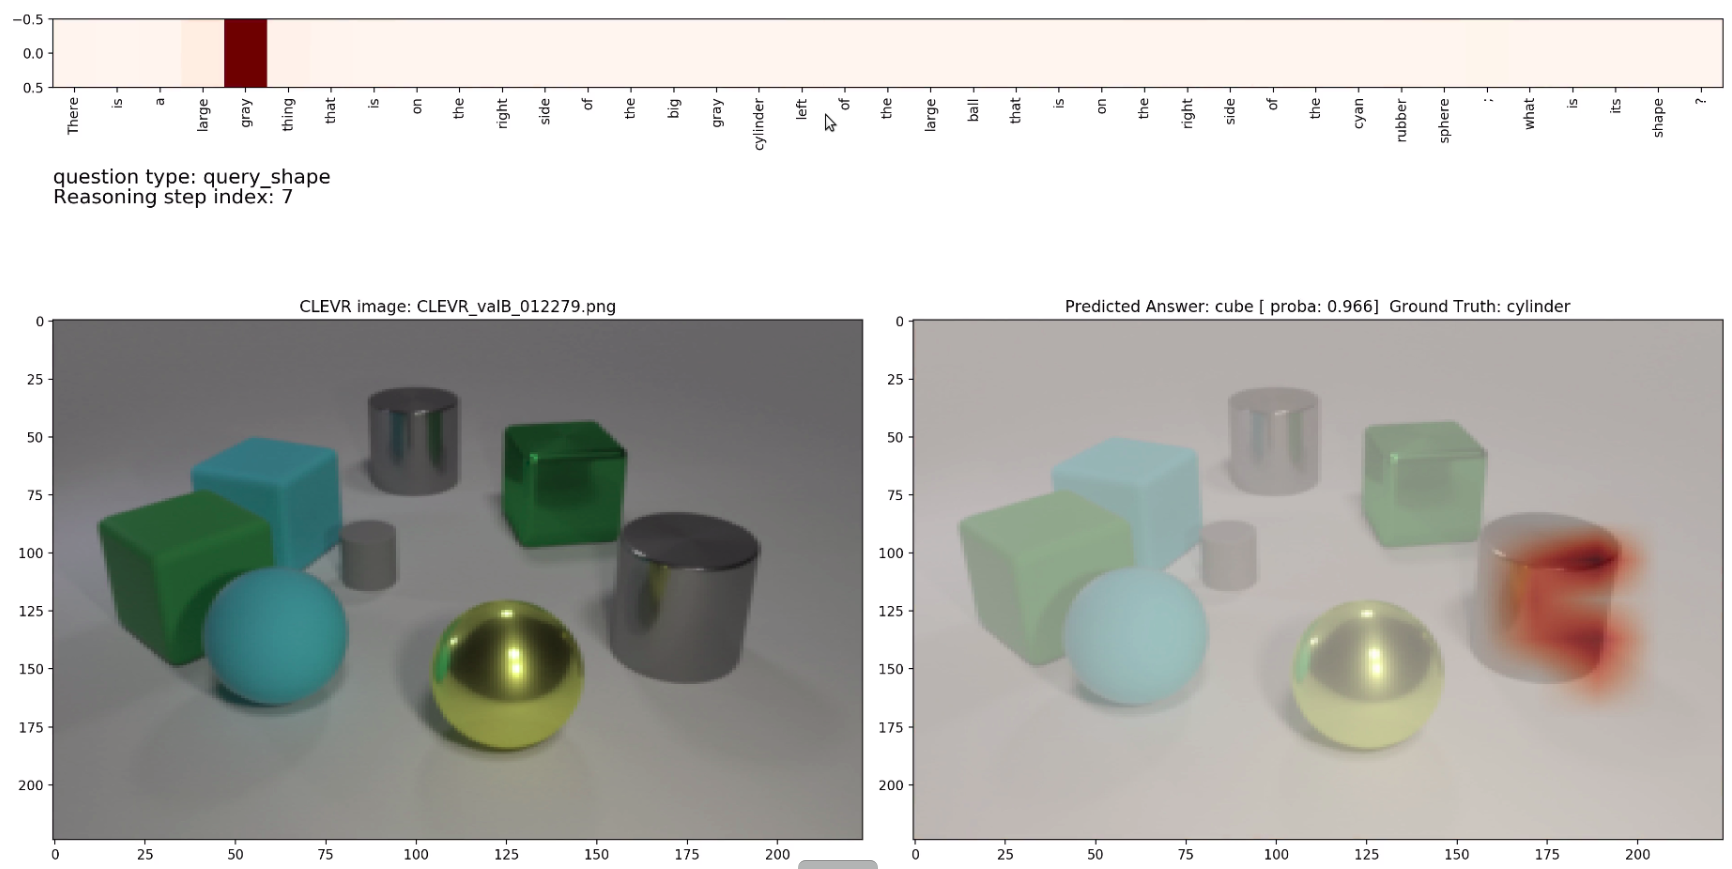
\includegraphics[width=\textwidth]{img/fail_mac_cogent_b_shape.png}
	\caption{The question reads as: \textit{There is a large gray thing that is on the right side of the big gray cylinder left of the large ball that is on the right side if the cyan rubber sphere; what is its shape?}}
	\label{fig:fail_mac_shape}
\end{figure}

\begin{figure}[]
	\centering
	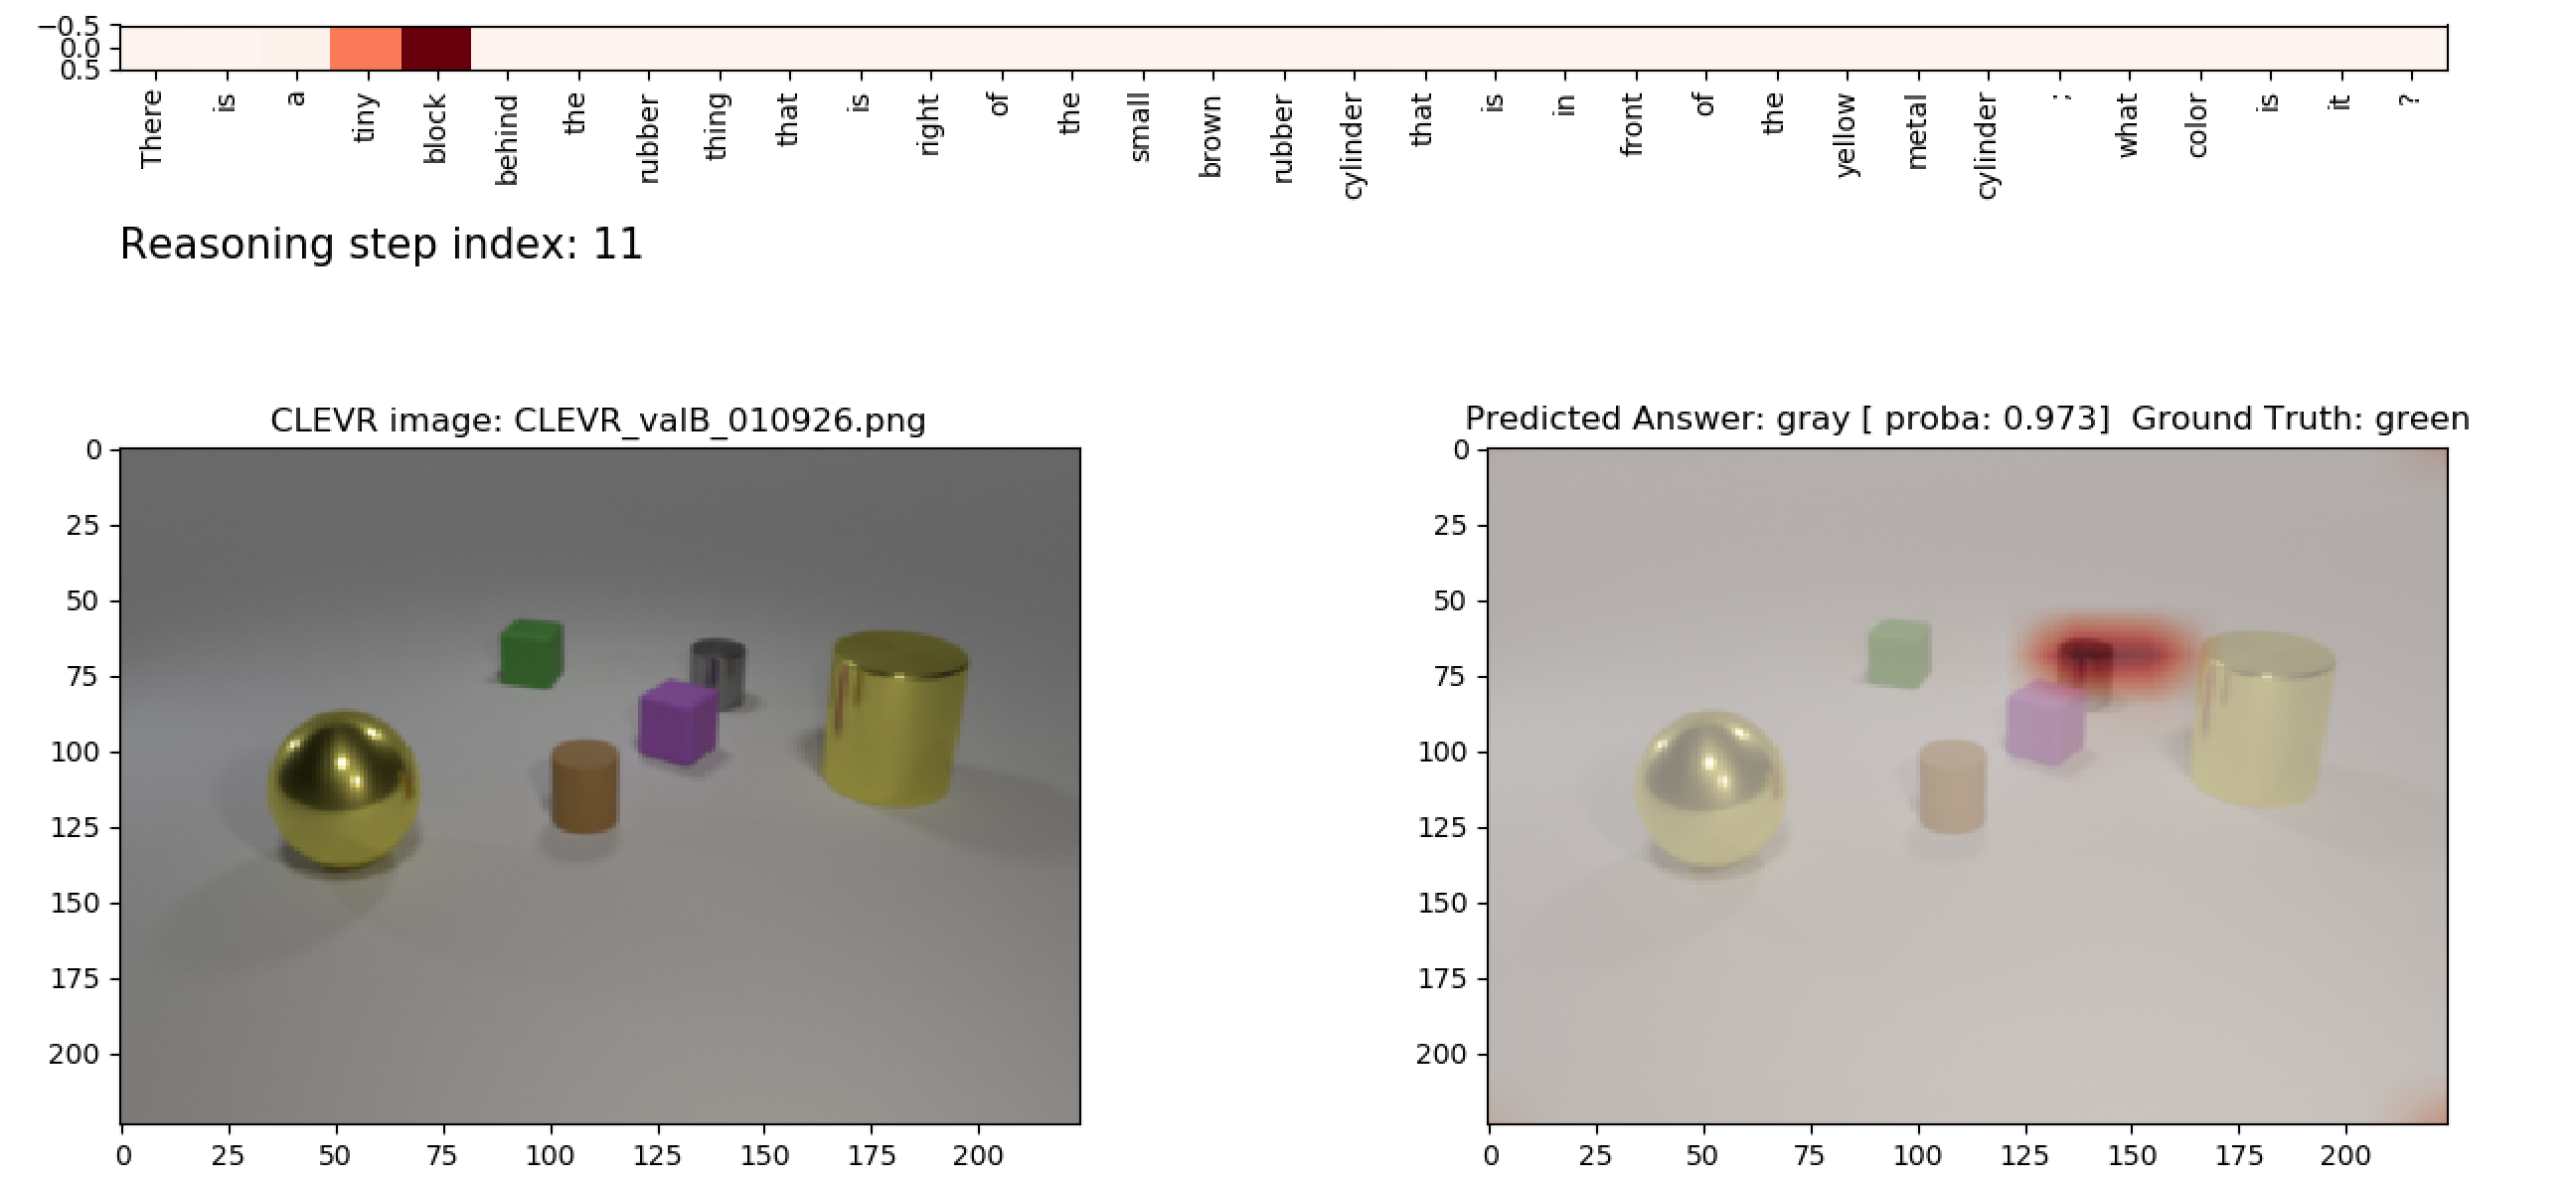
\includegraphics[width=\textwidth]{img/fail_mac_cogent_b_color.png}
	\caption{The question reads as: \textit{There is a tiny block behind the rubber thing that is right if the small brown rubber cylinder that is in front of the yellow metal cylinder; what color is it?}}
	\label{fig:fail_mac_color}
\end{figure}

\fig{fig:fail_mac_shape} presents a question where the model is asked about the shape of the leftmost gray cylinder. The model correctly finds it, as we can see from its visual attention map, and appears to refer to it using its color (\textit{gray}), as we can see from the attention of the question words. Yet, it defaults to predicting the shape as \textit{cube}, because it never saw gray cylinders during training, but instead saw gray cubes.

\fig{fig:fail_mac_color} presents a similar case, where the model is questioned about the color of the green cube at the back. MAC misses that object, and instead focuses on the nearby gray cylinder. We can hypothesize that MAC missed the green cube as it did not see this combination during training, and thus default to a combination that it knows.

Those examples indicate that MAC did not correctly separate the concept of shape from the concept of color, but have a better understanding of the colors (as it found the object of interest in \fig{fig:fail_mac_shape} by its color). This could come from that fact that the shape \textit{sphere} is associated with all possible colors in the dataset. 
